\documentclass[letterpaper,10pt]{article}
\usepackage{standalone}
\usepackage[spanish]{babel}
\usepackage[utf8]{inputenc}
\usepackage{ragged2e}
\usepackage{graphicx}
\usepackage[binary-units]{siunitx}
\usepackage{amsthm}% http://ctan.org/pkg/amsthm
\usepackage[left=2.5cm, top=2.5cm, right=2.5cm, bottom=3cm]{geometry}
\usepackage{lastpage}
\usepackage{fancyhdr}
\usepackage{listings}
\usepackage{multicol}
\usepackage{hyperref}
\usepackage{color}
\usepackage{placeins}
\definecolor{aliceblue}{rgb}{0.94, 0.97, 1.0}
\definecolor{mygreen}{rgb}{0.40, 0.67, 0.3}
\definecolor{antiquewhite}{rgb}{0.98, 0.92, 0.84}
\usepackage{pgfplots}
\pgfplotsset{compat=newest}
%% the following commands are needed for some matlab2tikz features
\usetikzlibrary{plotmarks}
\usetikzlibrary{arrows.meta}
\usepgfplotslibrary{patchplots}
\usepackage{grffile}
\usepackage{amsmath}

\usepackage{listings}
\usepackage{lstautogobble} % Fix relative indenting
\renewcommand{\lstlistingname}{Listado}
\lstset{
	backgroundcolor={\color{aliceblue}},basicstyle={\small \ttfamily},breaklines=true,captionpos=b,commentstyle={\color{mygreen}},emph={[1]{for,end,break}},emphstyle={[1]\color{red}},frame=tb,identifierstyle={\color{black}},keywordstyle={\color{blue}},language=Matlab,morekeywords={[2]{1}},numbers=left,numbersep=9pt,numberstyle={\tiny \color{black}},showstringspaces=false,stringstyle={\color{red}}}
\usepackage[shortlabels]{enumitem}

\pagestyle{fancy}
\renewcommand{\headrulewidth}{0pt}
\fancyhf{}% clear all fields
\fancyfoot[C]{\thepage\ de \pageref{LastPage}}

\setlength{\parskip}{3pt}

\begin{document}	
\begin{titlepage}
	\begin{figure}[h!]
		\begin{center}
			\vspace{1.5cm}
			% Aquí se inserta un escudo o emblema:
			
\includegraphics[scale= .5, ]{encabezado.png}
			\label{escudouam1}
			\vspace{-1cm}
		\end{center}
	\end{figure}
	\begin{center}
		\vspace{1cm} 
		\LARGE{\textbf{INSTITUTO TECNOLOGICO DE MORELIA}} \\
		\vspace{1cm}
		DEPARTAMENTO DE INGENIERIA ELECTRONICA
		DIVISIÓN DE ESTUDIOS PROFESIONALES \\  
		%nombre del prof
		\vspace{2.3cm} {\large \textbf{MATERIA}\\ \LARGE TELECOMUNICACIONES}
		
		% Incrementamos el interlineado
		%TEMA
		
		\vspace{1.5cm} {\large \textbf{TEMA}\\ \LARGE RADIO DIGITAL}\\ 
		
		\vspace{1.5cm} {\large \textbf{PROFESOR}\\ \LARGE JULIO JORGE MARQUEZ LUNA}
		
		\vspace{1.5cm} {\large \textbf{ALUMNO}\\ \large JORGE ALBERTO OCHOA LOPEZ} \\
		\normalsize{7º semestre
			%fecha
			\hfill {19/9/17}}\\ 
		MORELIA, MICHOACÁN
	\end{center}
\end{titlepage}
\pagebreak
\justify
\tableofcontents
\pagebreak
\pagenumbering{arabic}
	
	\section{INTRODUCCION:}
	El objetivo de esta práctica, era lograr analizar un sistema de control para un tanque que tiene un flujo de
	agua en la entrada y un flujo de agua de salida, los factores que determinan si el nivel del agua aumenta o decrece 
	es la capacidad del tanque comparada con la oposición al flujo de agua que va a dar una llave que hay a la salida.
	Para esto tuvimos que obtener la ecuación del balance de energía del sistema hidráulico, después realizamos una analogía 
	de esta ecuación hacia un circuito eléctrico con una fuente de corriente debido a que la analogía de flujo de agua
	es el flujo de corriente eléctrica. Ya que obtuvimos esta ecuación, aplicamos \textit{Laplace} para obtener una forma muy parecida
	a la ecuación proporcionada por \texttt{scilab}.\\
	
	Para realizar nuestra propia función que nos graficará la respuesta del sistema hidráulico partimos de la función de 
	la función de transferencia dada en la práctica, a la cual le agregamos una variable más, para hacerla similar a
	la ecuación de \texttt{scilab}, por medio de fracciones parciales y aplicando \textit{Laplace} inversa obtuvimos la ecuación con respuesta en 
	el tiempo para el sistema hidráulico. Finalmente propusimos valores de flujo de entrada y de salida para obtener los valores
	constantes de las ecuaciones y poder graficar las tres posibles respuestas del sistema.\\
	PAra poder entender este sistema mas concretamente utilizamos una analogía a un circuito Figura \ref{fig:circ}.
	
	\begin{figure}[h!]
		\centering
		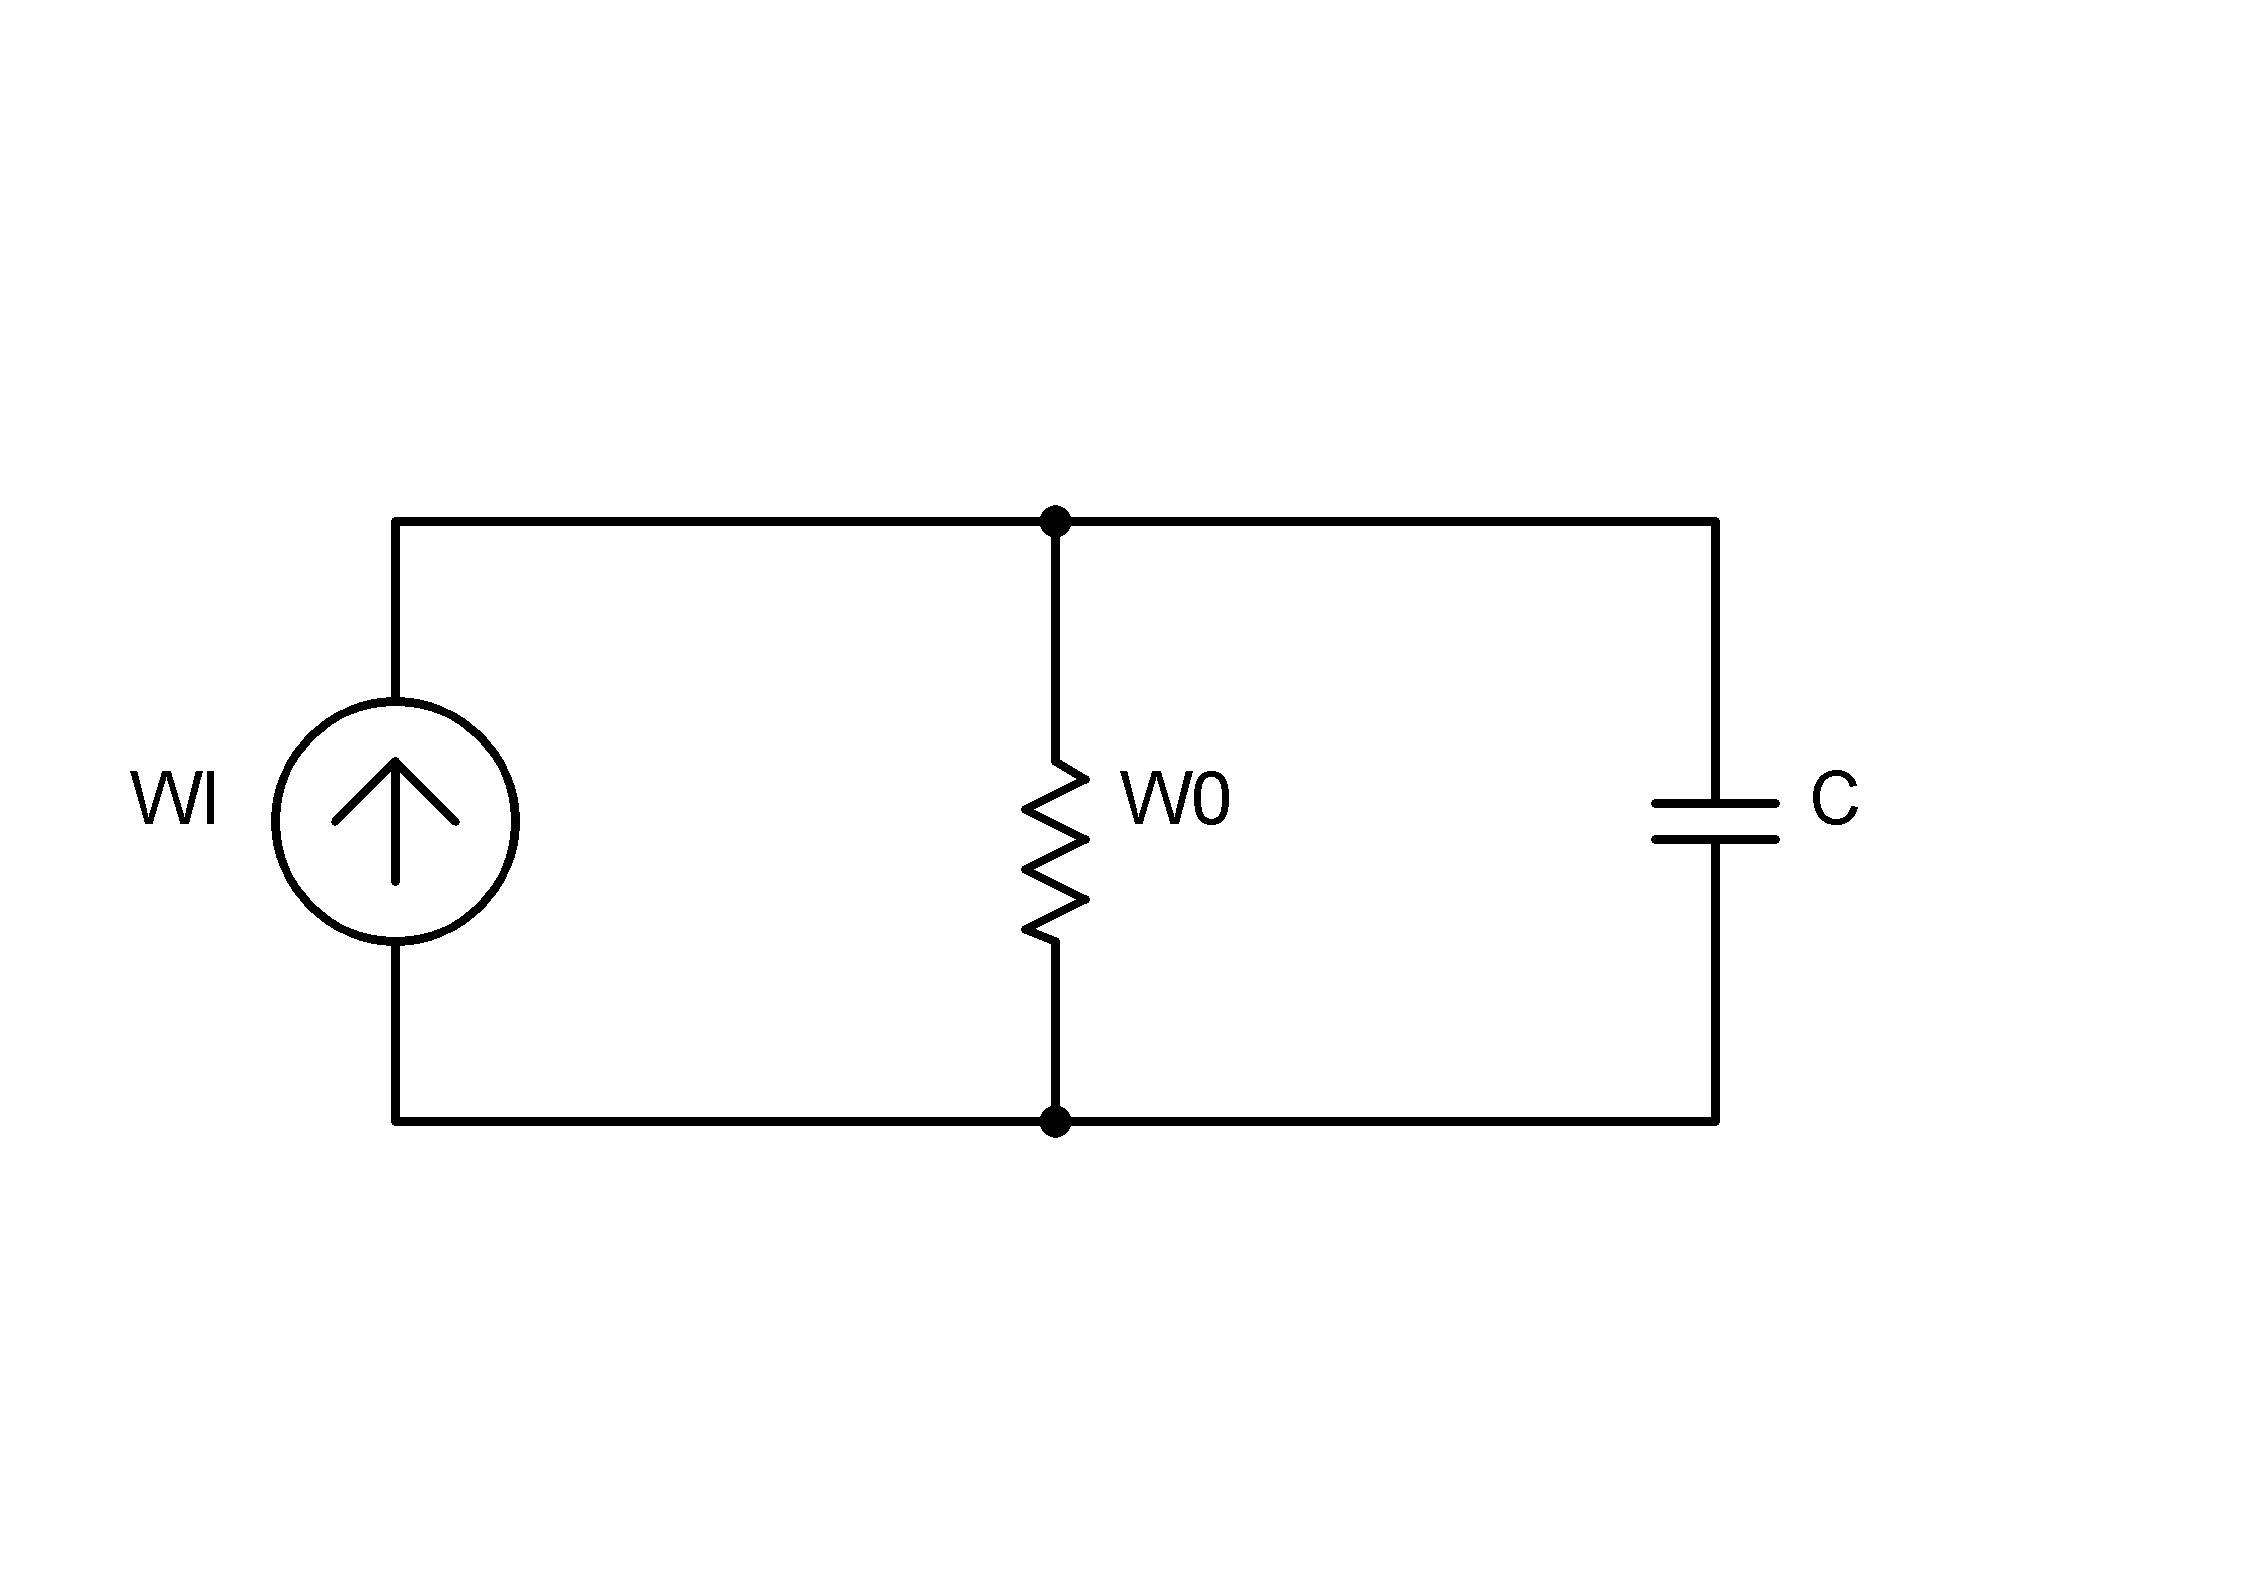
\includegraphics[width=0.4\linewidth]{circ}
		\caption{}
		\label{fig:circ}
	\end{figure}
	
	\section{METODOLOGIA:}
	\subsection{Parte 1}
	Lo primero que se hizo en la práctica fue considerar una función de transferencia genérica de primer orden que seria:
	\[H(s)=\frac{bs+c}{s+a}\]
	donde las letras a,b y c son números reales. Después se le aplica la función escalón unitario para ver su respuesta en el tiempo, esto queda de la forma:
	\[Y(s)=\frac{1}{s}\frac{bs+c}{s+a}\]
	a la cual se le aplicaran fracciones parciales, para esto se reescribe como:
	\[Y(s)=\frac{A}{s}\frac{B}{s+a}\]
	Resolviendo por fracciones parciales:
	\[bs+c=A(s+a)+Bs\]
	\[bs+c=(A+B)s+Aa\]
	\[A+B=b\]
	\[Aa=c\]
	por lo que tenemos los coeficientes A y B como:
	\begin{itemize}
		\item $A=\frac{c}{a}$
		\item $B=b-\frac{c}{a}$
	\end{itemize}
Después de obtener estos valores se sustituyen en la ecuación inicial y para obtener su función de transferencia \textbf{FT} se le aplica \textit{Laplace} inversa:
\[\mathcal{L}^{-1}=\{\frac{\frac{c}{a}}{s}+\frac{b-\frac{c}{a}}{s+a}\}\]
Con lo que obtenemos finalmente la función para implementar en \texttt{scilab} y ver que da una respuesta parecida a la de la función ya implementada en el programa
\[\frac{c}{a}+(b-\frac{c}{a})\exp{-at} \]
Finalmente al graficar esta función podemos corroborar que es correcta pues la respuesta es igual a la respuesta de la función creada por \texttt{scilab}
\pagebreak 
	\subsection{Parte 2}
	En esta parte nosotros creamos nuestra propia función mucho mas completa, la que se comparara con la función creada en el programa.\\
	Se ha agregado una variable extra a nuestra función de transferencia genérica para tomar en cuenta el termino $\tau$\\
	\[\frac{1}{s}(\frac{bs+c}{a+sd})\]
	A continuación hacemos lo que se hizo en la primer parte, que fue utilizar fracciones parciales para después aplicar \textit{Laplace} inversa y obtener la función con la que se trabajará
	\[bs+c=\frac{A}{s}+\frac{B}{a+sd}\]
	Se resuelven las fracciones parciales para los coeficientes A y B:
	\[bs+c=A(a+sd)+B(s)\]
	\[bs+c=Aa+Asd+Bs\]
	Finalmente obtenemos los valores de los coeficientes:
	\[b=Ad+B\]
	\[c=Aa\]  \[A=\frac{c}{a}\]
	\[b=\frac{cd}{a}+B\]
	\[B=b-\frac{cd}{a}\]
	Por lo tanto la respuesta de las fracciones parciales es:
	\[\frac{c}{sa}+\frac{\frac{b-cd}{a}}{a+sd}\]
	Y la transformada inversa de \textit{Laplace} quedaría de la forma:
	\[\mathcal{L}^{-1}=\{  \frac{c}{as}+\frac{\frac{b}{d}+\frac{c}{a}}{\frac{a}{d}+s}\} \]
	Que resolviendo queda:
	\[\frac{c}{a}+(\frac{b}{d}-\frac{c}{a}) \mathcal{} ^{-\frac{a}{d}t}\]
	Este resultado es nuestra función que gratificaremos mediante un código en \texttt{scilab} del cual compararemos las gráficas con las generadas por la función predeterminada del programa.
	\section{CÓDIGOS IMPLEMENTADOS}
	Primeramente mostraremos el codigo de la función predeterminada de \texttt{scilab} y sus gráficas cuando la salida del tanque 
	\section{CONCLUSIONES:}
	



	
	
	
%	\lstinputlisting[label={lst:graf14},caption={Código para generar la gráfica del polinomio de taylor de orden $12$ contra el error absoluto de éste. Se utilizo un intervalo de $0<x<pi$ para mejor visualización}]{mfc.m}
\section{Conclusiones}
Al querer obtener la respuesta en el tiempo de un sistema, es muy importante conocer todas las variables que lo
afectan y cuales dependen de otras, esto para poder obtener la ecuación del balance de energía del sistema, a la 
hora de realizar los cálculos nos fue mucho más fácil comprender cómo es que funcionaba el sistema al realizar la
analogía con un circuito eléctrico. En el primer caso donde el flujo de entrada era igual al flujo de salida
no obtenemos ninguna gráfica, esto debido a que solo obtenemos la función escalón, la cuál teóricamente tiene una 
amplitud que tiende a infinito en un tiempo igual a cero, es por eso que al graficar este caso, no obtenemos un gráfico.
\end{document}